
\section{2. Puente de Wien - Medici\'on de frecuencias}


El puente de Wien es un tipo de puente que consiste en dos capacitores y cuatro resistores. El mismo puede utilizarse para el cálculo de frecuencias lográndose la siguiente condición de balance:


\begin{figure}[H]
\begin{center}
\begin{circuitikz}
	
	\node [](Vg){}; 
	\draw (Vg) to[american voltage source , l = $V_g$] ++(0, -6) to[short] ++(4.5, 0);	
	\draw (Vg) to[short] ++(1.5, 0) node[](begin){} to[C, l =$C_1$] ++(0, -1.5) to[R, l = $R_1$] ++(0, -1.5) node[](vdl){};
	\draw (vdl) to[short] ++(0, -0.5) node[](parallel){};
	\draw (parallel) to[short] ++(1.25,0) to[R, l = $R_3$] ++(0, -2) to[short] ++(-1.25,0);
	\draw (parallel) to[C, l = $C_3$] ++(0, -2) to[short] ++(0, -0.5) node[ground]{};
	
	\draw (begin) to[short] ++(3,0) to[R, l = $R_2$] ++(0, -3) to[R, l = $R_4$] ++(0, -3);
	\draw (vdl) to[short] ++(3,0);
	

\end{circuitikz}
	\caption{Puente de Wien}
	\label{fig:Wien}
\end{center}
\end{figure}

\begin{equation}
f = \frac{1}{2\pi\sqrt{R_1R_3C_1C_3}}
\end{equation}

Para el caso en el que $R_1 = R_3$ y $C_1 = C_3$ la igualdad se simplifica:

\begin{equation}
f = \frac{1}{2\pi RC}
\end{equation}

con $R$ y $C$ el valor de los componentes.


En general se busca ajustar los valores de $R_1$ y $R_3$ para que coincidan y as\'i se cumpla la condici\'on de puente.

Asimismo se debe considerar $R_2 = 2 \cdot R_4$ para que se cumpla dicha condici\'on.

%%agregar aca sensibilidades 
\subsection{Diseno y elecci\'on de componentes}

Los componentes fueron seleccionados realizando c\'alculos para que el puente pueda estabilizarse en el rango de frecuencias solicitado ($100Hz$ a $2KHz$). De esta forma se tiene la siguiente distribuci\'on, tomando en cuenta las suposiciones realizadas con anterioridad.

\begin{table}[H]
    \centering
    \begin{tabular}{c c c c}
        $C_1 = C_3$ & $R_2 = 2 \cdot R_4$ & $R_1 = R_3 (preset)$ \\
        \hline \\
        $33 nF$ & $10 K\Omega$ & $50 K\Omega$ \\
        \hline
    \end{tabular}
\end{table}

Cabe destacar que se consider\'o un cierto margen en el rango de frecuencias, teniendo en cuenta las tolerancias de los componentes.



\subsubsection{Sensibilidades}
Se calcul\'o la sensibilidad del puente respecto a los componentes que se eligi\'o variar ($R_1$ y $R_3$).

La sensibilidad respecto de $R_1$ se puede calcular como:

\begin{equation}
\Delta V_d = \frac{Z_3 \cdot (Z_2+Z_4) - Z_4(Z_1 + \Delta Z_1 + Z_3)}{(Z_1+Z_3) \cdot (Z_2+Z_4)} \cdot v_g
\end{equation}
 
Veamos que

\begin{equation}
\frac{|\Delta Z_1|}{|Z_1|} = \frac{\Delta R_1}{|Z_1|} = \frac{\frac{\Delta R_1}{R_1}}{\sqrt{1+\frac{1}{(\omega \cdot C_1 \cdot R_1)^2}}}
\end{equation}

Suponiendo $\frac{1}{\omega \cdot C_1 \cdot R_1} >> 1$ obtenemos:

\begin{equation}
\frac{|\Delta Z_1|}{Z_1} = \frac{|\Delta R_1|}{R_1} \cdot \omega \cdot C_1 \cdot R_1
\end{equation}


Sabiendo esto, y asumiendo condici\'on de puente y $v_g$ unitario obtenemos

\begin{equation}
\Delta V_d = \frac{-A}{(A+1)^2} \cdot \omega \cdot R_1 \cdot C_1 \cdot \frac{\Delta R_1}{R_1}
\end{equation}

Donde $A = \frac{R_2}{R_4}$ es el factor cabeza de puente, y esta relaci\'on fue fijada con anterioridad. 

Asumiendo los valores de la tabla de selecci\'on de componentes, se grafica la sensibilidad para el rango de frecuencia.

\begin{figure}[H]
    \centering
    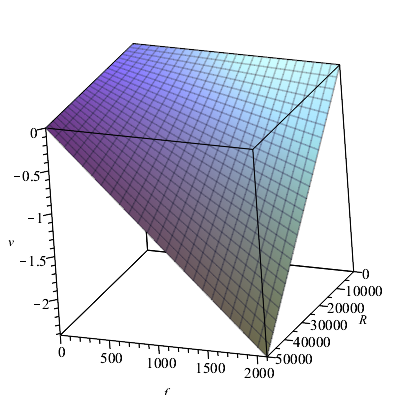
\includegraphics[width=0.9\textwidth]{Recursos/sensib_R1.png}
	\caption{Sensibilidad del circuito respecto a $R_1$}
   	\label{fig:sensib_R1}
\end{figure}

Se realiza un procedimiento an\'alogo para obtener la sensibilidad del puente respecto a $R_3$.

Veamos que:

\begin{equation}
Z_3 + \Delta Z_3 = \frac{R_3 + \Delta R_3}{1+S \cdot C_3 \cdot (R_3 + \Delta R_3)} 
\end{equation}

Suponemos $R_3 >> \Delta R_3$ y despreciamos los efectos de $\Delta R_3$ sobre el denominador debido a que est\'a multiplicado por un n\'umero relativamente peque\~no para el rango de frecuencias.

Luego se tiene

\begin{equation}
Z_3 + \Delta Z_3 = \frac{R_3}{1+S \cdot C_3 \cdot R_3} + \frac{\Delta R_3}{1+S \cdot C_3 \cdot R_3} = Z_3 + \frac{\Delta R_3}{1+S \cdot C_3 \cdot R_3}.
\end{equation}

Por lo que $\Delta Z_3 = \frac{\Delta R_3}{1+S \cdot C_3 \cdot R_3}$

Operando, se llega a la siguiente equivalencia:

\begin{equation}
\frac{|\Delta Z_3|}{|Z_3|} = \frac{\Delta R_3}{R_3}
\end{equation}

Finalmente, considerando $V_g$ unitario,

\begin{equation}
\Delta V_d = \frac{A}{(A+1)^2} \cdot \frac{\Delta R_3}{R_3}
\end{equation}

Por lo que ser\'a constante independientemente de la frecuencia ($V_d = \frac{2}{9}$).


\subsection{Mediciones}

Para la medici\'on del puente se utiliz\'o el mult\'imetro de banco. Con el mismo es posible medir niveles de tensi\'on que ser\'ian indistinguibles del ruido en un osciloscopio. Se estimul\'o al circuito con una senal de $5V_{pp}$ y se ajustaron los dos potensi\'ometros hasta obtener la menor tensi\'on posible:


\begin{table}[H]
\centering
\begin{tabular}{lllll}
Frecuencia del generador & Preset R\_1(Ohm) & Preset R\_2(Ohm) & Frecuencia calculada & Error(\%) \\ \hline
100                      & 46100            & 45915             & 104.83              & 3,92      \\
500                      & 9390             & 9175             & 519,6             & 4,83      \\
750                      & 6283             & 6219             & 771,55               & 2,87      \\
1000                     & 4695             & 4689             & 1027,89              & 2,79      \\
1250                     & 3833             & 3762             & 1270                 & 1,61      \\
1500                     & 3144             & 3125             & 1538,65              & 2,58      \\
1750                     & 2704             & 2665             & 1795,6               & 2,66      \\
2000                     & 2331             & 2318             & 2074,8               & 3,74     \\ \hline
\end{tabular}
\end{table}

En primer lugar se observa el comportamiento esperado respecto a las resistencias, para medir una frecuencia más cercana al límite inferior de la escala propuesta se precisan resistencias mayores. Además de lo anterior es importante hacer notar que el balance se logra solamente cuando ambos potenciómetros poseen resistencias casi iguales. Este balance no fue ideal, ya que no pudo llegarse a una diferencia de potencial igual a 0 entre ambas ramas, en cambio se tomó como $0$ el menor valor posible dada la frecuencia medida. Dicha tensión fue siempre menor a $10mV$. Dado el voltaje con el que se estimuló al circuito y el error porcentual obtenido  puede cdecirse que los resultados son satisfactorios y queda poco lugar para mejoras. Incluir las resistencias equivalentes de los capacitores utilizados tanto como las capacitancias parásitas de las resistencias es una de esas mejoras. No obstante, dadas las frecuencias en las que se trabajó, las capacitancias y las resistencias parásitas son despreciables en comparación a las tolerancias reales de los componentes. 




\subsection{Conclusiones}

Como conclusi\'on se puede destacar que se notaron diferencias entre el modelo te\'orico del puente y las mediciones realizadas en la pr\'actica. Principalmente se observa que es muy dificil equilibrar el puente en su totalidad, debido a las variaciones en los presets de ajuste y las tolerancias asociadas a los componentes del circuito.